\resizebox{.8\linewidth}{!}{%
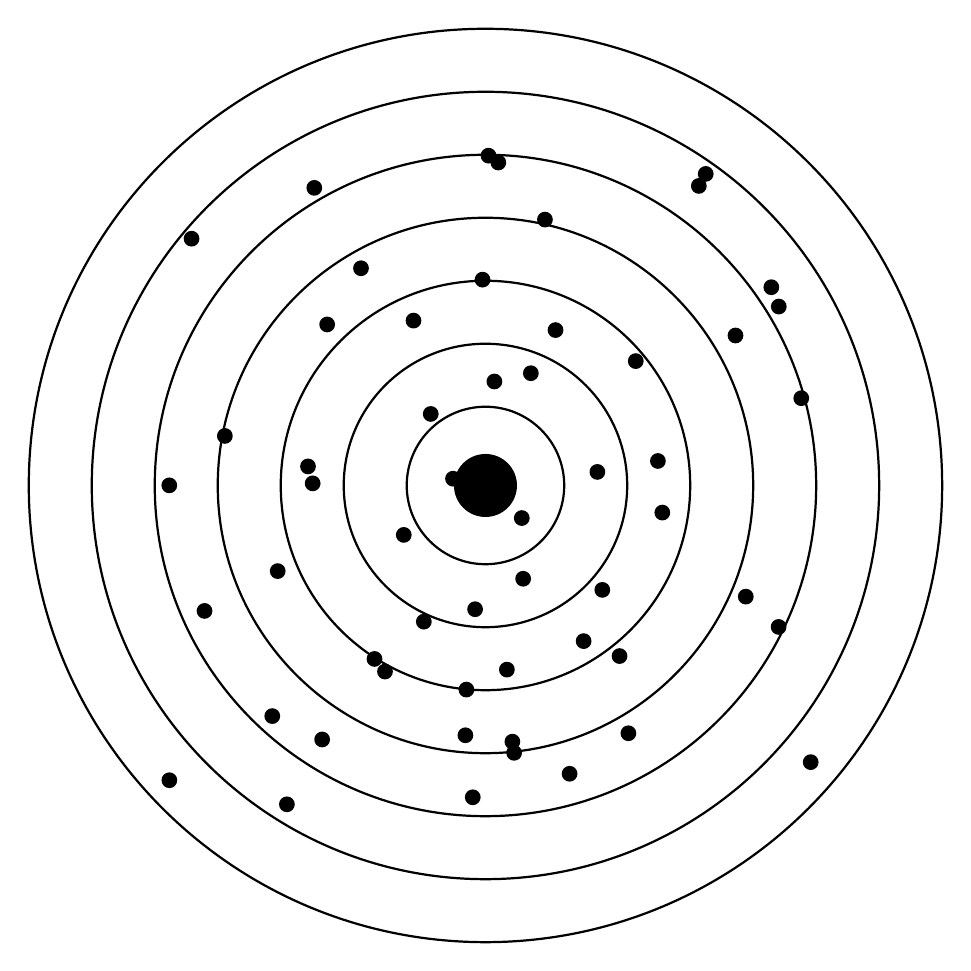
\begin{tikzpicture}
\def\farbea{black}
\def\farbeb{white}
\def\farbefill{\fuellung}
% mit verschiedenen ringen
%\foreach \x/\y in {  6/\farbea, 5/\farbeb, 4/\farbea, 3/\farbeb, 2/\farbea, 1/\farbeb} 
%{\draw[thick, fill=none, draw=black] (0,0) circle (\x cm);}

\foreach \x in { 1,1.8,...,6} 
{\draw[thick, fill=none, draw=black] (0,0) circle (\x cm);}

\draw[thick, fill=black, draw=none] (0,0) circle (.4 cm);

%oben rechts, reliable
% \def\shiftx{3}
% \def\shifty{3}
% \pgfmathsetseed{24122015}
% \foreach \p in {1,...,55}
% { \fill [\farbefill](1.3*rand+\shiftx,1.3*rand+\shifty) circle (0.1);
% }


%überall zerstreut
 \def\shiftx{0}
 \def\shifty{0}
 \pgfmathsetseed{24122015}
 \foreach \p in {1,...,55}
 { \fill [\farbefill](4.2*rand+\shiftx,4.2*rand+\shifty) circle (0.1);
 }


% %oberhalb zerstreut
% \def\shiftx{0}
% \def\shifty{2.5}
% \pgfmathsetseed{24122015}
% \foreach \p in {1,...,55}
% { \fill [\farbefill](3.4*rand+\shiftx,2.7*rand+\shifty) circle (0.1);
% }

%mittig alle
%\def\shiftx{0}
%\def\shifty{0}
%\pgfmathsetseed{24122015}
%\foreach \p in {1,...,55}
%{ \fill [\farbefill](1*rand+\shiftx,1*rand+\shifty) circle (0.1);
%}


\end{tikzpicture}

}